\documentclass[conference,10pt]{IEEEtran}
\usepackage[T1]{fontenc}
\usepackage{amsmath,amssymb,booktabs,array,url,graphicx}
\usepackage{tikz}
\usetikzlibrary{arrows.meta,positioning,calc}
\usepackage{flushend}
\usepackage[hidelinks]{hyperref}
\hypersetup{pdftitle={A CHIA Loop for ECC Optimization with Routed Feedback},pdfauthor={Ssu-Rui Lee}}
\title{A CHIA Loop for ECC Optimization\\with Routed Feedback}
\author{\IEEEauthorblockN{Ssu-Rui Lee}\IEEEauthorblockA{RaydioTek, Taiwan\\\texttt{ssr.lee@raydiotek.tw}}}
\begin{document}
\maketitle
\raggedbottom
\brokenpenalty=10000
\begin{abstract}
We build a CHIA loop that uses routed measurements to select function-preserving changes to error-correcting-code (ECC) decoders. A runtime language model chooses a local edit or decides whether to evaluate a supplied plan; deterministic tools apply the change, prove equivalence, and return physical measurements. Starting from already optimized feasible designs, the normalized three-workload energy score falls from 0.9914 to 0.8952 for 64-bit payloads and from 0.8844 to 0.7955 for 32-bit payloads: reductions of 9.70\% and 10.05\%. Final delays are 2.3741 and 2.0816\,ns, below the same 2.40\,ns limit. Intermediate results explain the gains: measured timing failures lead to broader path protection and repair, while extending binary parity operations to three-input gates opens a new search space. Energy uses routed parasitics and functional activity; it is not measured silicon power.
\end{abstract}

\section{Introduction}

% P01
Equivalent Boolean expressions can have different physical costs. In an ECC decoder, complementing an internal parity signal and compensating its consumers preserves the external outputs, yet changes cell types, loads, and routed timing. A low-energy candidate may expose a new critical path. Finding a useful successor then requires the path and workload evidence, as well as the aggregate score.

% P02
We implement that process in CHIA~\cite{chia}, a framework for agentic hardware/software co-design. The loop's state is a verified, routed circuit with its measurements. A model selects a bounded experiment, CHIA executes the transformation and evaluators, and the returned evidence informs the next choice (Fig.~\ref{fig:loop}). Outer developers also use these reports to extend the operations between episodes.

% P03
We contribute \textbf{an executed CHIA loop} with reusable, equivalence-checked parity operations; \textbf{decision trajectories} linking measured failures to later choices; and \textbf{two hardware findings}: newly exposed timing paths changed which phase assignments were feasible, while admitting three-input parity consumers expanded a fixed-boundary binary space whose two-input exclusive-NOR count had reached a certified minimum. Table~\ref{tab:milestones} traces the improvements from earlier register-transfer-level (RTL) search and physical-tuning results.

\begin{figure}[!t]
\centering
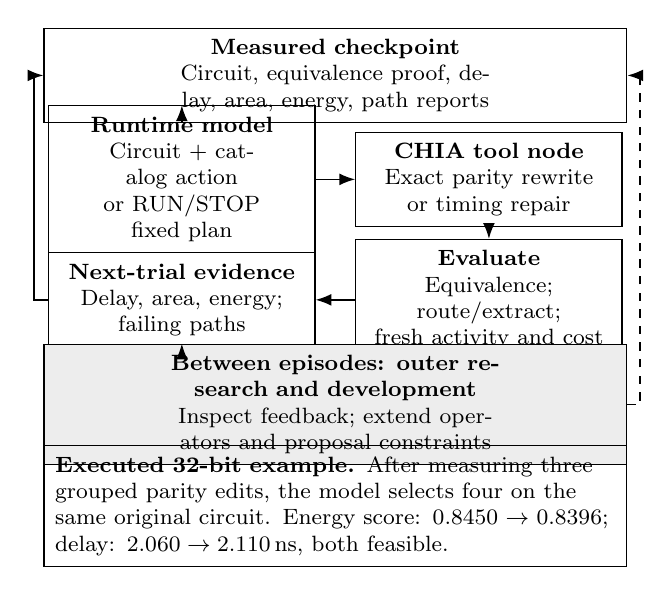
\begin{tikzpicture}[x=1cm,y=1cm,>=Latex,
 box/.style={draw,align=center,font=\footnotesize,inner sep=4pt},
 process/.style={box,text width=3.10cm,minimum height=.92cm},
 flow/.style={->,line width=.6pt},outer/.style={->,dashed,line width=.6pt}]
\node[box,text width=7.12cm] (archive) at (0,0) {\textbf{Measured checkpoint}\\Circuit, equivalence proof, delay, area, energy, path reports};
\node[process] (agent) at (-1.95,-1.32) {\textbf{Runtime model}\\Circuit + catalog action\\or RUN/STOP fixed plan};
\node[process] (edit) at (1.95,-1.32) {\textbf{CHIA tool node}\\Exact parity rewrite\\or timing repair};
\node[process] (eval) at (1.95,-2.85) {\textbf{Evaluate}\\Equivalence; route/extract;\\fresh activity and cost};
\node[process] (result) at (-1.95,-2.85) {\textbf{Next-trial evidence}\\Delay, area, energy;\\failing paths};
\draw[flow] (archive.south -| agent.north)--(agent.north);
\draw[flow] (agent)--(edit);\draw[flow] (edit)--(eval);\draw[flow] (eval)--(result);
\draw[flow] (result.west)--++(-.18,0)|-(archive.west);
\node[box,fill=black!7,text width=7.12cm] (development) at (0,-4.18) {\textbf{Between episodes: outer research and development}\\Inspect feedback; extend operators and proposal constraints};
\draw[outer] (result.south)--(development.north -| result.south);
\draw[outer] (development.east)--++(.16,0)|-(archive.east);
\node[box,text width=7.12cm,align=left] at (0,-5.47) {\textbf{Executed 32-bit example.} After measuring three grouped parity edits, the model selects four on the same original circuit. Energy score: $0.8450\to0.8396$; delay: $2.060\to2.110$\,ns, both feasible.};
\end{tikzpicture}
\caption{A completed evaluation feeds the next decision. The example is an observed runtime choice; gray separates development of new operations from use of existing operations. Coordinator-executed timing queries can enrich the feedback outside the local controller's RUN/STOP interface.}
\label{fig:loop}
\end{figure}


% P04
CHIA's processor case study feeds timing reports into successive iterations~\cite[Sec.~5.3]{chia}. Dr. RTL~\cite{drrtl} uses critical-path analysis and parallel RTL rewriting; RTLScout~\cite{rtlscout} combines code and synthesis optimization. Our narrower setting exposes the operation, exact circuit parent, returned measurement, and next decision for parity-rich ECC logic, including cases where conventional repair and new rewrites are complementary.

\begin{table*}[!t]
\centering
\caption{Measured milestones before and after local and global optimization. Every row reports one complete candidate under the same width-specific evaluation.}
\label{tab:milestones}
\fontsize{9}{10.4}\selectfont
\setlength{\tabcolsep}{5.0pt}
\begin{tabular}{@{}lrrrrrr@{}}
\toprule
Design / operation & Delay (ns) & Area ($\mu$m$^2$) & Stress & Uniform & Low-toggle & $E_{\mathrm{norm}}$\\
\midrule
\multicolumn{7}{@{}l}{\textbf{64-bit decoder}}\\
Searched RTL reference$^{\dagger}$ & 2.526346 & 2392 & 2.541008 & 2.027927 & 0.435884 & 1.000000\\
\textbf{RTL + physical tuning (start)} & 2.372445 & 2434 & 2.641683 & 2.010297 & 0.412100 & 0.991375\\
Pin swaps, downsizing, and tree rotation & 2.358853 & 2416 & 2.625896 & 2.008364 & 0.410271 & 0.987614\\
Batched local phase refinements & 2.371359 & 2416 & 2.577747 & 1.964015 & 0.387134 & 0.955592\\
Shared-consumer phase refinement & 2.398144 & 2416 & 2.570336 & 1.956617 & 0.381644 & 0.948946\\
Fold for additional timing headroom & 2.363135 & 2427 & 2.583333 & 1.958906 & 0.382310 & 0.951466\\
Feedback-recovered local design & 2.362535 & 2427 & 2.534646 & 1.911262 & 0.375450 & 0.932080\\
Multi-path-protected global assignment & 2.376334 & 2427 & 2.476977 & 1.859091 & 0.354799 & 0.899342\\
Power-weighted global assignment & 2.369255 & 2427 & 2.474160 & 1.856980 & 0.353019 & 0.897156\\
Feedback-selected local pair & 2.375917 & 2427 & 2.472119 & 1.854769 & 0.353273 & 0.896767\\
\textbf{Final three-input refinement} & \textbf{2.374088} & \textbf{2425} & \textbf{2.470199} & \textbf{1.854112} & \textbf{0.351798} & \textbf{0.895180}\\
\midrule
\multicolumn{7}{@{}l}{\textbf{32-bit decoder}}\\
Masked-RTL reference & 2.248806 & 1836 & 1.595185 & 1.140097 & 0.327811 & 1.000000\\
\textbf{Projected searched RTL (start)} & 2.049337 & 1299 & 1.379291 & 0.974656 & 0.306806 & 0.884433\\
Transferred local phase pairs & 2.061026 & 1299 & 1.363067 & 0.959193 & 0.297479 & 0.867296\\
Three-star local trial & 2.060426 & 1299 & 1.339273 & 0.937648 & 0.286393 & 0.844951\\
Feedback-selected four-star trial & 2.110139 & 1299 & 1.331617 & 0.930286 & 0.284876 & 0.839637\\
Minimum-count binary assignment & 2.069854 & 1299 & 1.280010 & 0.889243 & 0.267722 & 0.799553\\
Power-weighted binary assignment & 2.098243 & 1299 & 1.279071 & 0.886069 & 0.266960 & 0.797646\\
Mixed-arity single-group trial & 2.080952 & 1297 & 1.277263 & 0.886224 & 0.267330 & 0.797686\\
\textbf{Final mixed-arity assignment} & \textbf{2.081588} & \textbf{1296} & \textbf{1.275677} & \textbf{0.883614} & \textbf{0.266264} & \textbf{0.795511}\\
\midrule
\multicolumn{7}{@{}l}{\textbf{Starting design $\rightarrow$ final:} 64-bit energy score $-9.70\%$, area $-0.37\%$, delay $+1.643$\,ps;}\\
\multicolumn{7}{@{}l}{32-bit energy score $-10.05\%$, area $-0.23\%$, delay $+32.251$\,ps. Both final designs satisfy the same delay limit.}\\
\bottomrule
\end{tabular}\par
\vspace{3pt}
\begin{minipage}{.96\textwidth}\footnotesize Energy columns are pJ/vector: unrestricted encoded-bit patterns (Stress), uniform valid codewords (Uniform), and valid codewords from single-bit-changing payloads (Low-toggle). $E_{\mathrm{norm}}$ is their geometric-mean energy ratio to the reference of the same width (Eq.~\eqref{eq:energy}). \emph{Start} identifies the pre-optimized feasible comparison designs. $^{\dagger}$The 64-bit reference alone fails the 2.40\,ns limit. Row order does not imply direct ancestry. Decimal places preserve tool output, not confidence bounds.\end{minipage}
\end{table*}


\section{Loop, Operations, and Evaluation}
\subsection{Decisions and deterministic execution}

% P05
In local episodes, the runtime model receives eligible circuits, legal edits, previous outcomes, and available diagnostics. It chooses a circuit and edit or stops. In fixed-plan episodes, it chooses RUN or STOP for one supplied circuit--plan pair. The recorded models are Gemini 3.8 Flash and Gemini 3.1 Pro Preview~\cite{gemini}. CHIA schedules evaluation nodes through Ray~\cite{ray}, a distributed execution framework. A completed result returns correctness, delay, area, workload energies, and timing evidence. Failed-timing circuits remain available for repair; only verified feasible results can improve the best feasible score.

% P06
Outer coordinators and coding agents build new operators, protection constraints, and global plans. Earlier model-requested timing queries were executed by the coordinator, outside the local controller's RUN/STOP schema. Tools evolve between episodes. Sibling trials share a circuit parent while later decisions can use earlier trial feedback.

\subsection{Parity operations and checking}

% P07
For a parity gate $g$, let $b_g=0$ denote exclusive OR (XOR) and $b_g=1$ exclusive NOR (XNOR). A phase $p_n\in\{0,1\}$ complements net $n$ when set. With input nets $I(g)$ and output $o$, the required new gate polarity is
\begin{equation}
 b'_g=b_g\oplus p_o\oplus\bigoplus_{i\in I(g)}p_i.
 \label{eq:phase}
\end{equation}

% P08
External ports and unsupported consumers have fixed phase. A \emph{pair} changes two connected gates; a \emph{star} changes a producer and all its parity consumers. Global assignments handle overlapping choices. XOR2/XNOR2 and XOR3/XNOR3 name two- and three-input cells. Path protection fixes selected phases or cell polarities. For power-weighted proposals, parent-derived internal-power weights rank assignments; they are proxies, not predictions of a candidate's energy. Small components are solved exactly; larger proposals use bounded simulated annealing. Polarity-sensitive mapping is established prior work~\cite{phase}; our contribution concerns its checked use and physical feedback in this loop.

% P09
The functional reference is Common Cells' \texttt{cc\_ecc\_decode}~\cite{commoncells}, revision \texttt{121182ea}, retaining data, syndrome, and status outputs. Yosys~\cite{yosys} proves each valid child equivalent to its checked parent for defined two-state inputs. OpenROAD~\cite{openroad} edits and routes the circuit; OpenRCX~\cite{openrcx} extracts parasitics. Icarus Verilog~\cite{icarus} generates functional activity, and OpenSTA~\cite{opensta} uses that activity, parasitics, and cell-library models for power and timing. A final circuit may reuse its own new pre-route proof when netlist bytes and proof context are identical.
\subsection{Measurements and comparison starts}

\begin{figure*}[t]
\centering
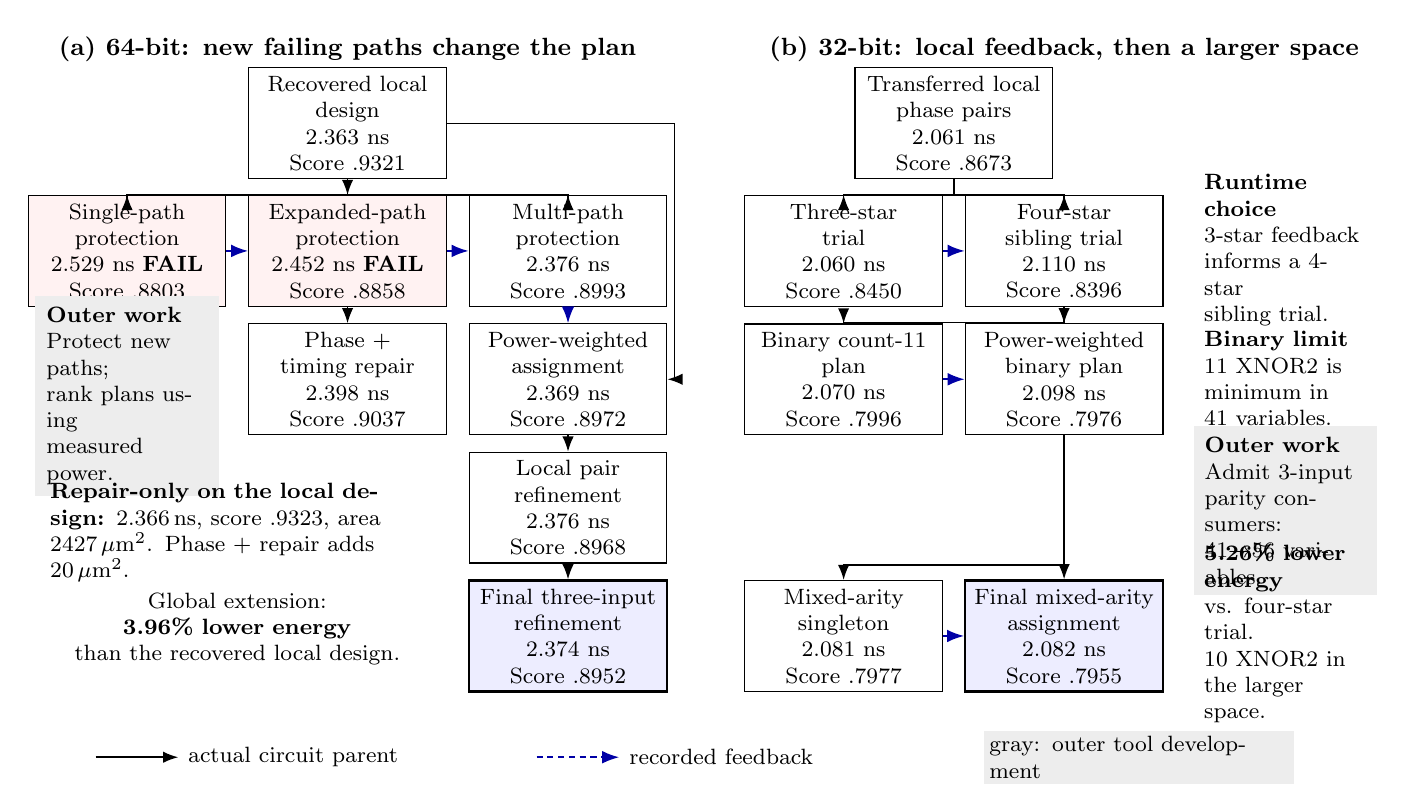
\begin{tikzpicture}[x=1cm,y=1cm,>=Latex,
 design/.style={draw,align=center,text width=2.30cm,minimum height=1.08cm,inner sep=3pt,font=\footnotesize},
 fail/.style={design,fill=red!5},final/.style={design,fill=blue!7,line width=.85pt},
 parent/.style={->,line width=.55pt},info/.style={->,dashed,draw=blue!65!black,line width=.7pt,dash pattern=on 2.2pt off 1.7pt},
 note/.style={fill=black!7,align=left,text width=2.05cm,inner sep=4pt,font=\footnotesize}]
\begin{scope}
\node[font=\small\bfseries] at (2.8,.94) {(a) 64-bit: new failing paths change the plan};
\node[design] (bbf) at (2.8,0) {Recovered local\\design\\2.363 ns\\Score .9321};
\node[fail] (H1) at (0,-1.62) {Single-path\\protection\\2.529 ns \textbf{FAIL}\\Score .8803};
\node[fail] (H2) at (2.8,-1.62) {Expanded-path\\protection\\2.452 ns \textbf{FAIL}\\Score .8858};
\node[design] (J1) at (5.6,-1.62) {Multi-path\\protection\\2.376 ns\\Score .8993};
\node[design] (I1) at (2.8,-3.25) {Phase +\\timing repair\\2.398 ns\\Score .9037};
\node[design] (N1) at (5.6,-3.25) {Power-weighted\\assignment\\2.369 ns\\Score .8972};
\node[design] (N2) at (5.6,-4.88) {Local pair\\refinement\\2.376 ns\\Score .8968};
\node[final] (S2) at (5.6,-6.51) {Final three-input\\refinement\\2.374 ns\\Score .8952};

\draw[parent] (bbf.south)--++(0,-.20)-|(H1.north);
\draw[parent] (bbf.south)--(H2.north);
\draw[parent] (bbf.south)--++(0,-.20)-|(J1.north);
\draw[parent] (bbf.east)--(6.95,0)|-(N1.east);
\draw[info] (H1.east)--(H2.west);
\draw[info] (H2.east)--(J1.west);
\draw[parent] (H2.south)--(I1.north);
\draw[info] (J1.south)--(N1.north);
\draw[parent] (N1.south)--(N2.north);
\draw[parent] (N2.south)--(S2.north);
\node[note] at (0,-3.46) {\textbf{Outer work}\\Protect new paths;\\rank plans using\\measured power.};
\node[align=left,text width=4.48cm,font=\footnotesize,anchor=north west] at (-1.10,-4.45) {\textbf{Repair-only on the local design:} 2.366\,ns, score .9323, area 2427\,$\mu$m$^2$. Phase + repair adds 20\,$\mu$m$^2$.};
\node[font=\footnotesize,align=center,text width=4.5cm] at (1.4,-6.42) {Global extension: \textbf{3.96\% lower energy}\\than the recovered local design.};
\end{scope}
\begin{scope}[xshift=9.1cm]
\node[font=\small\bfseries] at (2.8,.94) {(b) 32-bit: local feedback, then a larger space};
\node[design] (G0) at (1.4,0) {Transferred local\\phase pairs\\2.061 ns\\Score .8673};
\node[design] (G1) at (0,-1.62) {Three-star\\trial\\2.060 ns\\Score .8450};
\node[design] (ff6) at (2.8,-1.62) {Four-star\\sibling trial\\2.110 ns\\Score .8396};
\node[design] (O1) at (0,-3.25) {Binary count-11\\plan\\2.070 ns\\Score .7996};
\node[design] (O2) at (2.8,-3.25) {Power-weighted\\binary plan\\2.098 ns\\Score .7976};
\node[design] (V1) at (0,-6.51) {Mixed-arity\\singleton\\2.081 ns\\Score .7977};
\node[final] (V2) at (2.8,-6.51) {Final mixed-arity\\assignment\\2.082 ns\\Score .7955};

\draw[parent] (G0.south)--++(0,-.20)-|(G1.north);
\draw[parent] (G0.south)--++(0,-.20)-|(ff6.north);
\draw[info] (G1.east)--(ff6.west);
\draw[parent] (ff6.south)--++(0,-.20)-|(O1.north);
\draw[parent] (ff6.south)--(O2.north);
\draw[info] (O1.east)--(O2.west);
\draw[parent] (O2.south)--++(0,-1.65)-|(V1.north);
\draw[parent] (O2.south)--(V2.north);
\draw[info] (V1.east)--(V2.west);
\node[align=left,text width=2.06cm,font=\footnotesize] at (5.61,-1.61) {\textbf{Runtime choice}\\3-star feedback\\informs a 4-star\\sibling trial.};
\node[align=left,text width=2.06cm,font=\footnotesize] at (5.61,-3.24) {\textbf{Binary limit}\\11 XNOR2 is\\minimum in\\41 variables.};
\node[note] at (5.61,-4.92) {\textbf{Outer work}\\Admit 3-input\\parity consumers:\\41$\to$56 variables.};
\node[align=left,text width=2.06cm,font=\footnotesize] at (5.61,-6.48) {\textbf{5.26\% lower energy}\\vs. four-star trial.\\10 XNOR2 in\\the larger space.};
\end{scope}
\draw[parent] (-.4,-8.05)--(.65,-8.05) node[right,font=\footnotesize] {actual circuit parent};
\draw[info] (5.2,-8.05)--(6.25,-8.05) node[right,font=\footnotesize] {recorded feedback};
\node[note,text width=3.8cm,minimum height=.22cm,inner sep=2pt] at (12.85,-8.05) {gray: outer tool development};
\end{tikzpicture}
\caption{Selected feedback episodes after local refinement. Solid arrows identify circuit parents; dashed arrows carry measured feedback to a later decision or outer proposal development. Gray marks outer development. Score denotes normalized energy $E_{\mathrm{norm}}$ (Eq.~\eqref{eq:energy}); FAIL marks delay above 2.40\,ns. The earlier stages and raw workload energies are in Table~\ref{tab:milestones}.}
\label{fig:trajectory}
\end{figure*}


% P10
The decoders correct single-bit errors and detect double-bit errors for 64-bit or 32-bit payloads. We use the SkyWater 130-nm high-density library~\cite{sky130} at the typical corner, 1.8\,V and 25\,$^\circ$C, 0.05\,ns input slew, and 0.005\,pF output load. Acceptance requires maximum external-output delay no greater than 2.40\,ns. Routing targets 2.575\,ns; setup repair targets 2.35\,ns. Cell area is reported separately.

% P11
Each search workload contains 1,024 vectors spaced 10\,ns apart, seed 2026092101: unrestricted encoded-input bits, encoded uniform payloads, or encoded payloads changing one bit per vector. Total estimated power $P_w$ includes internal, switching, and leakage components. For the observed window $T=10.24\,\mu$s, energy per vector and its aggregate are
\begin{equation}
 E_w=P_wT/1024,\qquad
 E_{\mathrm{norm}}(x)=\left[\prod_{w=1}^{3}\frac{E_w(x)}{E_w(\mathrm{ref})}\right]^{1/3}.
 \label{eq:energy}
\end{equation}

% P12
Each width has its own fixed energy reference (Table~\ref{tab:milestones}); cross-width scores are not absolute efficiency comparisons. Both references are in-project RTL variants; the 64-bit reference fails timing. Our headline starts instead from the feasible \emph{RTL + physical tuning} and \emph{projected searched RTL} rows, and includes all later refinements. The workload activity lacks delay back-annotation, so these are routed-parasitic energy estimates without glitch-accurate timing.


\section{Results: From Tuned Designs to Further Gains}
\subsection{Where the comparison designs came from}

% P13
The 64-bit start already incorporates RTL search, timing repair, and power recovery. In a three-route episode over existing RTL candidates, two choices fail at 2.4320 and 2.4075\,ns; after receiving those results, the model selects a third existing RTL candidate, which reaches 2.3799\,ns. Subsequent downsizing of two inverters and rerouting produces the 2.372445\,ns starting design. Pin swaps, selective downsizing, and tree rotation then create the lower-energy, higher-headroom checkpoint shown in Table~\ref{tab:milestones}. The first pin-swap experiment is a direct tool-execution prototype outside CHIA; its successor and the reported downstream results run through CHIA.

% P14
Local parity search reduces the score further, but progress is not monotonic. A shared-consumer edit leaves only 1.856\,ps margin; absorbing an inverter into a stronger parity cell restores timing headroom while increasing energy and area. Later, a four-star batch fails timing. A conservative single-star trial succeeds; after receiving the failed batch's path diagnosis, the runtime selects a two-star successor, producing the \emph{feedback-recovered local design}. It is retained for 37.465\,ps margin, although other local branches have slightly lower scores and less margin.

% P15
The 32-bit start is a fixed width projection of previously searched RTL, using radix-2 parity trees and a reversible XOR recombination of syndrome bits. This transfer is prescribed by the outer coordinator. It already cuts energy score by 11.56\% and area by 29.25\% versus the project's mask-based parity reference. Transferring the 64-bit power-recovery recipe makes zero cell-size changes and preserves its metrics. Local phase pairs nevertheless reduce energy. The model then tries three stars and, after reading their measurements, four stars on the same original circuit. That second trial lowers all three energy estimates but adds 49.713\,ps delay relative to the first; its score is 0.839637.
\subsection{Timing feedback and conventional repair}

% P16
Figure~\ref{fig:trajectory} separates circuit ancestry from feedback. On the 64-bit local design, protecting only the old critical path reduces XNOR2 count from 60 to 18 and energy score to 0.880345, but a new path reaches 2.528992\,ns. Adding the newly exposed cone in a sibling plan improves delay to 2.452134\,ns, still infeasible. Conventional repair makes this phase plan feasible at 2.398176\,ns and score 0.903709. Repair alone on the earlier local circuit returns 2.365566\,ns and 0.932320. The composition has lower energy, with 20\,$\mu$m$^2$ more area and less timing margin than that control.

% P17
Using the measured failing and near-limit paths, outer development protects 34 phase variables and 33 gate polarities. The resulting global assignment keeps 37 XNOR2 cells and meets timing at score 0.899342. A power-weighted sibling from the same local circuit keeps that count but reaches 0.897156. Feedback-selected pair refinement and two XOR3-to-XNOR3 replacements yield the final 0.895180 result. The last edit improves its direct parent by 0.1770\%; the full extension beyond the local design improves it by 3.96\%.
\subsection{A larger representation on the 32-bit decoder}

% P18
Binary global assignment lowers XNOR2 count from 31 to 11. A count-11 witness and a Yosys Boolean satisfiability (SAT) check rejecting count $\leq10$ establish the minimum within the exact 41-variable, fixed-boundary binary representation. A power-weighted sibling has the same count and lower measured energy. Both start from the four-star design.

% P19
Outer development then admits three-input parity consumers, expanding the representation to 56 phase variables. A single-group trial improves area and delay but slightly worsens the energy score. After reading that tradeoff, the runtime chooses RUN for a supplied global plan on the same parent. The supplied plan comes from bounded annealing with an area-first proxy and an XNOR2-count tie-breaker. Its nine cell changes leave 10 XNOR2 and seven XNOR3 cells, outside the old certificate's scope. Delay, area, and all three energy estimates improve over the direct parent. The last step gains 0.2677\%; the extension beyond the four-star result gains 5.26\%.
\subsection{Full before/after and retained tradeoffs}

% P20
From the pre-optimized starts, normalized energy falls 9.70\% and 10.05\%, with area reductions of 9 and 3\,$\mu$m$^2$. Final delay increases by 1.643 and 32.251\,ps, respectively, but both remain feasible. Against the masked-RTL reference, the final 32-bit design also has 20.45\% lower energy score, 29.41\% less area, and 167.218\,ps less delay. These comparisons use the same observations and explicitly different starting rows; they are not additive gains.

% P21
A later undo restores the final 64-bit netlist and placement, then produces a different route with score 0.894859 and 1.800\,ps more delay. We retain this physical result separately from the logic refinement. Another repaired branch offers 2.370334\,ns, 2424\,$\mu$m$^2$, and score 0.896634. No single design is best in every column.

\section{Limits and Reuse}

% P22
Recorded feedback shows what was available and what choice followed; it does not establish a model-policy advantage. An earlier equal-budget comparison gives each arm 12 post-synthesis queries and four logical route queries. Neither Flash nor a fixed rule improves the shared 0.991375 incumbent; among new queries, the fixed rule reaches 1.034309 versus 1.046497 for Flash. This comparison predates the phase operators. The supplement separates follow-on budgets from earlier search and development.

% P23
The study uses one library corner and three search workloads, without held-out workloads or repeated-route confidence intervals. Equivalence and routed timing are not physical signoff. The supplied artifact includes saved-decision CHIA replay for the final 64-bit and 32-bit operations, historical result receipts, and a fixed-plan model gate. Earlier portability checks exercised both saved plans; the model-gate code is mock-tested; live endpoint use remains unvalidated. Code and results repository: \url{https://github.com/thisray/2026_CHIA_Hackathon}.
\section{Conclusion}

% P24
Routed feedback supported continued optimization after RTL search and physical tuning in these experiments: newly exposed paths prompted protection or repair, and a broader parity representation enabled further improvements. The measured gains retain timing feasibility, with failures and area/delay tradeoffs recorded alongside them.
\begin{thebibliography}{13}
\bibitem{chia} A. Cui \emph{et al.}, ``CHIA: An open-source framework for principled, agentic AI-driven hardware/software co-design research,'' arXiv:2606.27350v3, 2026.
\bibitem{drrtl} W. Fang \emph{et al.}, ``Dr. RTL: Autonomous agentic RTL optimization through tool-grounded self-improvement,'' arXiv:2604.14989v2, 2026.
\bibitem{rtlscout} F. Arnold, R. Amaudruz, D. Tsaras, R. Andri, and L. Cavigelli, ``RTLScout: Joint agentic code and synthesis optimization for efficient digital circuits,'' arXiv:2606.06530v2, 2026.
\bibitem{gemini} Google, ``Gemini models,'' model documentation, accessed Sep. 24, 2026. \url{https://ai.google.dev/gemini-api/docs/models}.
\bibitem{ray} P. Moritz \emph{et al.}, ``Ray: A distributed framework for emerging AI applications,'' in \emph{OSDI}, 2018, pp. 561--577.
\bibitem{phase} M. Zhao and S. S. Sapatnekar, ``Technology mapping algorithms for domino logic,'' \emph{ACM TODAES}, vol. 7, no. 2, pp. 306--335, 2002, doi: 10.1145/544536.544541.
\bibitem{commoncells} PULP Platform, ``Common Cells: \texttt{cc\_ecc\_decode},'' source code, accessed Sep. 24, 2026. \href{https://github.com/pulp-platform/common_cells/blob/121182eaa0fa1f67b74eaa97c73b8a7133adda6a/src/cc_ecc_decode.sv}{Source at revision \texttt{121182ea}}.
\bibitem{yosys} C. Wolf and J. Glaser, ``Yosys---A free Verilog synthesis suite,'' in \emph{Austrochip}, 2013.
\bibitem{openroad} T. Ajayi \emph{et al.}, ``Toward an open-source digital flow: First learnings from the OpenROAD project,'' in \emph{DAC}, 2019, pp. 76:1--76:4, doi: 10.1145/3316781.3326334.
\bibitem{openrcx} The OpenROAD Project, ``Parasitics extraction (OpenRCX),'' documentation, accessed Sep. 24, 2026. \url{https://openroad.readthedocs.io/en/latest/main/src/rcx/README.html}.
\bibitem{icarus} S. Williams and contributors, ``Icarus Verilog,'' documentation, accessed Sep. 24, 2026. \url{https://steveicarus.github.io/iverilog/}.
\bibitem{opensta} Parallax Software, ``OpenSTA,'' documentation, accessed Sep. 24, 2026. \url{https://openroad.readthedocs.io/en/latest/main/src/sta/README.html}.
\bibitem{sky130} Google and SkyWater Technology, ``SkyWater open source PDK,'' documentation, accessed Sep. 24, 2026. \url{https://skywater-pdk.readthedocs.io/en/main/}.
\end{thebibliography}

\section*{AI Assistance}

% P25
The human author set the research objectives, evaluation criteria, and resource boundaries; directed priorities; and critically reviewed the results and manuscript. AI research and coding agents assisted with literature, operator development, experiment coordination, analysis, and writing. Runtime Gemini decisions are separately identified in the methods and traces. The human author retains responsibility for the paper's claims, interpretation, tone, and quality.
\end{document}
